\chapter{Classification with Fundamental Models}

In this chapter we present the classification of one-dimensional discrete statistical models with rational maximum likelihood estimator (MLE) using fundamental models. The classification is due to Arthur Bik and Orlando Marigliano~\cite{bik2022classifying}. 

\begin{center}
    \textbf{Problem statement:} Can we find a class of easy to understand models that serve as building blocks for all one-dimensional discrete statistical models with rational MLE?
\end{center}
The answer to this question are \emph{reduced} and \emph{fundamental models}.

\section{Parametrization}

It turns out that one-dimensional discrete statistical models with rational MLE admit the following parametrization.

\begin{proposition}\label{prop:parametrization}
    Let \( \mathcal{M} \) be a one-dimensional discrete statistical models with rational maximum likelihood estimator. Then, there exists a map of the form
    \begin{gather*}
        p: [0,1] \to \Delta_n, \quad \theta \mapsto (w_k \theta^{i_k} (1-\theta)^{j_k})_{k=0}^n \\
        i_k, j_k \in \mathbb{Z}_{\geq 0}, \;  w_k \in \mathbb{R}_{> 0} \quad \forall k = 0, \dots, n
    \end{gather*}
    such that \( \mathcal{M} = \mathrm{image}(p) \).
\end{proposition}

We introduce some notation to simplify the proof of Proposition \ref{prop:parametrization}.
Let \( \mathcal{M} \subset \Delta_n \) be a one-dimensional discrete statistical model parametrized by rational functions \( p_0 =  \frac{g_0}{h_0}, \dots, p_n =  \frac{g_n}{h_n} \). Define \( b \) to be the least common multiple of \( h_0, \dots, h_n \) and \( a_i \coloneqq b p_i \). Since \( \sum p_k = 1 \), we can multiply by \( b \) to obtain \( \sum a_k = b \). We see that the polynomials \( a_0, \dots, a_n, b \) determine the statistical model \( \mathcal{M} \), and have no common factors. The log-likelihood function is then given by
\begin{align*}
    \ell(p) &= \sum u_i \log p_i \\
    &= \sum u_i \log \frac{a_i}{b} \\
    &= \sum u_i \log a_i - \sum u_i \log b.
\end{align*}
To find the maximum likelihood estimator, we need find all critical points of the log-likelihood function. This is equivalent to finding the roots of the gradient of the log-likelihood function
\begin{align}\label{eq:score-equations}
    \ell(p(\theta))' &= \sum u_k \frac{a_k'}{a_k} - \sum u_k \frac{b'}{b} = 0.
\end{align}
These equations are called the \emph{score equations} in algebraic statistics, and the number of complex solutions to these equations for general data \( u \in \mathbb{C}^{n + 1} \) is called the \emph{maximum likelihood degree} of the statistical model. This ML degree has an important meaning in algebraic statistics, as it determines the complexity of the model. We have the following relationship between the ML estimator and the ML degree.

\begin{proposition}\label{prop:rational-mle}
    Having rational maximum likelihood estimator can be expressed equivalently by saying that the maximum likelihood degree of the statistical model is one.
\end{proposition}

\begin{proof}
   Refer to \cite{duarte2021discrete} for a proof.
\end{proof}

To prove Proposition \ref{prop:parametrization}, we need the following lemma.

\begin{lemma}\label{lem:two-complex-factors}
    If \( \mathcal{M} \) has rational MLE, then there are exactly two distinct complex linear factors in \( a_0, \dots, a_n \), and \( b \).
\end{lemma}

\begin{proof}
    We prove the lemma in three steps:
    \begin{itemize}
        \item Let \( f \) be the product of all distinct complex linear factors in \( a_0, \dots, a_n, b \).  If we multiply the score equations \eqref{eq:score-equations} by \( f \), we get 
        \begin{align*}
            f \cdot \ell(p(\theta))' &= \sum u_k f \frac{a_k'}{a_k} - \sum u_k f \frac{b'}{b} = 0. 
        \end{align*}
        Note that every linear factor of \( a_k \) with multiplicity \( m \) occurs in \( a_k' \) with multiplicity \( m-1 \); thus every summand of \( \frac{a_k'}{a_k} \) is of the form \( \frac{\lambda}{(x-\xi)} \), where \( \lambda \in \mathbb{R} \) and \( x-\xi \) is some linear factor of \( a_k \); hence \( f \cdot  \frac{\lambda}{(x-\xi)}  \) is of degree \( \mathrm{deg}(f) - 1\), and therefore \( f \cdot \ell(p(\theta))' \) is of degree \( \mathrm{deg}(f) - 1\).

        \item We claim that the roots of \( \ell(p(\theta))' \) are the same as the roots of \( f \cdot \ell(p(\theta))' \). Assume we have shown this claim.  By Proposition \ref{prop:rational-mle} the ML degree is one. So, \( \ell(p(\theta))' \) has one root. Thus, \( f \cdot \ell(p(\theta))' \) has one root, and therefore \( f \cdot \ell(p(\theta))' \) is of degree one. This implies that \( \mathrm{deg}(f) = 2 \) with the previous step. Thus, there are exactly two distinct complex linear factors in \( a_0, \dots, a_n \), and \( b \).
        
        \item It remains to show that the roots stay the same. Clearly, every root of \( \ell(p(\theta))' \) is a root of \( f \cdot \ell(p(\theta))' \). Conversely, we want to show that no new roots are introduced when multiplying by \( f \), i.e. roots of \( f \) are not roots of \(  f \cdot \ell(p(\theta))' \). To do so, we rewrite 
        \begin{gather*}
            f \cdot \ell(p(\theta))' = \sum_{k=0}^n u_k f \frac{a_k'}{a_k} - \sum_{k=0}^n u_k f \frac{b'}{b} = \sum_{k=0}^{n + 1} v_k f \frac{c_k'}{c_k}\\
            v_k = u_k, \; c_k = a_k \quad \text{for } k = 0, \dots, n,\\ \quad v_{n+1} = - \sum_{k=0}^n u_k, \; c_{n+1} = b.
        \end{gather*}
        Let \( q \) be a complex linear factor of \( f \). We define polynomials \( r_0, \dots, r_{n+1} \) and \( r \) such that \( c_k = q^{l_k}r_k \), \( f = q r \), and \( r_0, \dots, r_{n+1}, r \) do not have \( q \) as a factor. Then, we have for \(  k = 0, \dots, n+1 \) that
        \begin{gather*}
            f \frac{c_k'}{c_k} = q r \cdot \frac{l_k q^{l_k - 1} q'r_k +  q^{l_k}r_k'}{q^{l_k}r_k} = q r\frac{l_k q' }{q} + q r\frac{r_k'}{r_k} \equiv rl_k q' \pmod q.
        \end{gather*}
        Thus, we obtain 
        \begin{align*}
            f \cdot \ell(p(\theta))' \equiv rq'\sum_{k=0}^{n + 1} v_k l_k \equiv rq' \sum_{k=0}^{n } v_k(l_k - l_{n+1}) \pmod q.
        \end{align*}
        Note that by definition of \( l_k \), a value of \( l_k = 0 \) means that \( q \) is not a factor of \( c_k \). By definition of \( f \), at least one \( l_k > 0 \). On the other hand, not all \( l_k \) can be positive since \( a_0, \dots, a_n, b \) share no common factors. Hence, not all \( l_k - l_{n+1} = 0 \) vanish. Hence, for generic data \( u \) we assume \( \sum_{k=0}^{n } v_k(l_k - l_{n+1}) \neq 0 \). This with \( q'r \not \equiv 0 \pmod q \) implies that \( q \) is not a complex linear factor of \( f \cdot \ell(p(\theta))' \). We showed that the roots of \( f \) are not roots of \( f \cdot \ell(p(\theta))' \).
    \end{itemize}
\end{proof}

Equipped with the lemma, we can now prove Proposition \ref{prop:parametrization}.

\begin{proof}
    We want to show the following parametrization of \( \mathcal{M} \):
    \begin{align*}
        p: [0,1] \to \Delta_n, \quad \theta \mapsto (w_k \theta^{i_k} (1-\theta)^{j_k})_{k=0}^n
    \end{align*}
    First, we show that \( I \) is a single closed real interval and not a union of closed intervals. For the sake of contradiction assume that \( I = \bigcup_{k} I_k \) is a union of closed disjoint intervals. By definition of \( \mathcal{M} \) we know that \( p(\partial I) \subset \partial \Delta_n \). Thus, there exist \( \theta_1, \theta_2 \in \partial I_0 \) and \( \theta_3, \theta_4 \in \partial I_1 \) with \( p_i(\theta_1) = p_i(\theta_2) =  0 \) and \( p_j(\theta_3) = p_j(\theta_4) = 0 \) for some \( i,j = 0, \dots, n \). Note that \( \theta_1, \theta_2 \) are roots of \( \frac{a_i}{b} \) and  \( \theta_3, \theta_4 \) are roots of \( \frac{a_j}{b} \). By Lemma \ref{lem:two-complex-factors} exactly two distinct complex linear factors occur in \( a_0, \dots, a_n, b \). Hence, \( \theta_3 = \theta_1 \) or \( \theta_3 = \theta_2 \). Contradiction for \( I_0 \) and \( I_1 \) are disjoint.

    The previous argument shows that \( I = [\alpha, \beta ]\) is a real single closed interval. Thus, the roots of \( a_0, \dots, a_n, b \) are real and take values in \( \partial I = \left\{ \alpha, \beta \right\} \). By a suitable parametrization, we can assume without loss of generality that \( I = [0,1] \). We can now write the polynomials \( a_0, \dots, a_n, b \) as
    \begin{align*}
        a_k(\theta) &= w_k \theta^{i_k} (1-\theta)^{j_k} \\
        b(\theta) &= w \theta^{i} (1-\theta)^{j}
    \end{align*}
    with \( w_k, w \in \mathbb{R}_{>0} \), and \( i_k, j_k, i, j \in \mathbb{Z}_{\geq 0} \) for all \( k = 0, \dots, n \). Since \( a_0, \dots, a_n, b \) share no common factors, there exists some \( i_k = 0 \) if \( i > 0 \); however this would contradict \(0 < w_k \leq a_0(0) + \dots + a_n(0) = b(0) = 0\). So \( i = 0 \). Similarly, \( j = 0 \). Finally, we divide \( p \) by \( w \) to obtain \( b \equiv 1 \).
\end{proof}

\begin{corollary}
    Any one-dimensional {discrete} {statistical} {models} with rational MLE can be represented by \( (w_k, i_k, j_k)_{k=0}^n \) for \( w_k \in \mathbb{R}_{>0} \) and \( i_k, j_k \in \mathbb{Z}_{\geq 0} \).
\end{corollary}

From now on, we only consider one-dimensional discrete statistical models with rational MLE; we call them \emph{models} for short.

\begin{definition}
    The degree \( \mathrm{deg}(\mathcal{M}) \) of a model \( \mathcal{M} \) represented by \( (w_k, i_k, j_k)_{k=0}^n \) is defined as \( \mathrm{max}\left\{ i_k + j_k : k = 0, \dots, n \right\} \).
\end{definition}

\begin{remark}\label{rem:equivalent-models}
    We view two models \( (w_k,i_k,j_k)_{k=0}^n \) and \( (w_k',i_k',j_k')_{k=0}^n \) as the same model if they are equal up to a permutation of the coordinates.
\end{remark}

\begin{example}
    The sequence \( ((1,0,2), (2,1,1), (1,2,0)) \) represents the binomial model with two trials. It has degree two. Its parametrization is given by \( \theta \mapsto ((1-\theta)^2, 2\theta(1-\theta),\theta^2) \). Also see Figure \ref{fig:binom-discrete-model} for a visualization of the binomial model within the probability simplex \( \Delta_2 \).

    Note that we view the sequences \( ((1,0,2), (2,1,1), (1,2,0)) \) or \( ((2,1,1), (1,0,2), (1,2,0)) \) as the same model as \( ((2,1,1), (1,2,0), (1,0,2)) \) since the order of the coordinates does not matter.
\end{example}

\begin{definition}
    Let \( \mathcal{M} \) be a model represented by \( (w_k, i_k, j_k)_{k=0}^n \). The set of exponent pairs \( (i_k, j_k)_{k=0}^n \) is called the support of \( \mathcal{M} \), denoted by \( \mathrm{supp}(\mathcal{M}) \).
\end{definition}

This was our first step towards understanding the structure of models. The next step is to introduce the concept of reduced models.

\section{Reduced Models}

Models in this section refer to one-dimensional discrete statistical models with rational MLE.

\begin{definition}
    We call a model represented by \( (w_k, i_k, j_k)_{k=0}^n \) \emph{reduced} if \( (i_k, j_k) \neq \mathbf 0 \) for all \( k = 0, \dots n \), and \( (i_k, j_k) \neq (i_l, j_l) \) for all \( k \neq l \).
\end{definition}

Due to \( (i_k, j_k) \neq (i_l, j_l) \), we can use functions to represent reduced models.

\begin{remark}\label{rem:representation-of-models-by-functions}
    A reduced model \( \mathcal{M} \) represented by \( (w_k, i_k, j_k)_{k=0}^n \) can also be identified by a function \( f: \mathbb{Z}^2 \to \mathbb{R}_{\geq 0}, (i, j) \mapsto w \), where \( w = w_k \) if \( (i_k, j_k) = (i, j) \) and \( w = 0 \) otherwise. The support of \( f \) is the set of all pairs \( (i, j) \) with \( f(i, j) > 0 \). It coincides with the support of \( \mathcal{M} \).
\end{remark}


Reduced models are our first building blocks for the classification of models. This statement is justified by the following two propositions. They show that every non-reduced model can be transformed into a reduced model by a sequence of linear embeddings.

\begin{proposition}\label{prop:linear-embedding-1}
    Let \( n \in \mathbb{N}_{>0} \).
    Let \( \mathcal{M} \) be a model represented by \( (w_k, i_k, j_k)_{k=0}^n \). If \( (i_l, j_l) = \mathbf{0} \) for some index \( l \), then there exist a model \( \mathcal{M}' \), \( \lambda \in [0,1] \) and \( k = 0, \dots, n \) such that
    \begin{align*}
        \mathcal{M} = \Psi_{\lambda,k}(\mathcal{M}'),
    \end{align*}
    where \( \Psi_{\lambda, k}: \Delta_{n-1} \to \Delta_n \) is defined as \(  p_i \mapsto \begin{cases}
        \lambda p_i & \text{if } k \neq i, \\
        1-\lambda & \text{if } k = i.
    \end{cases} \)
\end{proposition}

\begin{proof}
    Let \( (i_l, j_l) = \mathbf{0} \) for some index \( l \). If \( w_l = 1 \), then \( w_m = 0 \) for all \( m \neq l \); this contradicts \( w_m > 0 \) by Proposition \ref{prop:parametrization}. Set \( \lambda = 1 - w_l > 0 \) and \( k = l \). Define the model \( \mathcal{M}' \) represented by 
    \begin{align*}
        \left(\frac{w_h}{1-w_l}, i_h, j_h\right)^n_{h=0, h \neq l}.
    \end{align*}
    Then, \( \mathcal{M} = \Psi_{\lambda,k}(\mathcal{M}') \).
\end{proof}

\begin{proposition}\label{prop:linear-embedding-2}
    Let \( n \in \mathbb{N}_{>0} \).
    Let \( \mathcal{M} \) be model represented by \( (w_k, i_k, j_k)_{k=0}^n \). If \( (i_m, j_m) = (i_l, j_l)  \) for \( m \neq l \), then there exist a model \( \mathcal{M}' \), \( \lambda \in [0,1] \) and \( k,h = 0, \dots, n \) such that
    \begin{align*}
        \mathcal{M} = \Psi_{\lambda,k,h}(\mathcal{M}'),
    \end{align*}
    where \( \Psi_{\lambda, k,h}: \Delta_{n-1} \to \Delta_n \) is defined as \(  p_i \mapsto \begin{cases}
         p_i & \text{if } i \notin \left\{ k,h \right\}, \\
        \lambda p_k & \text{if } k = i, \\
        (1-\lambda) p_k & \text{if } h = i. \\
    \end{cases} \)
\end{proposition}

\begin{proof}
    Define \( \lambda = \frac{w_m}{w_m + w_l} \), \( k = m \), and \( h = l \). Define the model \( \mathcal{M}' \) represented by 
    \begin{align*}
        \left( w_g + \delta_{gm}w_l, i_g, j_g  \right)^n_{g=0, g \neq l}.
    \end{align*}
    Then, \( \mathcal{M} = \Psi_{\lambda,k}(\mathcal{M}') \).
\end{proof}

By repeatedly applying the two propositions, we can transform any model into a reduced model. 

\begin{corollary}\label{cor:reduced-models}
    If \( \Delta_n \) contains a model of degree \( d \), then there also exists a reduced model of degree \( d \) in \( \Delta_m \) for some \( m \leq n \).
\end{corollary}


\section{Fundamental Models}

As before, models refer to one-dimensional discrete statistical models with rational MLE. The main building blocks for the classification of models are \emph{fundamental models}; we will see that reduced models come from fundamental models.

\begin{definition}\label{def:fundamental-model}
    We call a model represented by \( (w_k, i_k, j_k)_{k=0}^n \) \emph{fundamental} if it is reduced and the equation \( p_0 + \dots p_n \equiv 1 \) for given \( (i_k, j_k)_{k=0}^n \) uniquely determines the weights \( (w_k)_{k=0}^n \).
\end{definition}

\begin{example}
    The binomial model with two trials is fundamental. Given \( (i_0, j_0) = (0,2) \), \( (i_1, j_1) = (1,1) \), and \( (i_2, j_2) = (2,0) \), the equation \( p_0 + p_1 + p_2 = w_0\theta^2 + w_1\theta(1-\theta) + w_2(1-\theta)^2 \equiv 1 \) uniquely determines the weights \( w_0 = 1, w_1 = 2, w_2 = 1 \). To see this observe that this equation is equivalent to \( w_0\theta^2 + w_1\theta - w_1 \theta^2 + w_2 -w_22\theta + w_2\theta^2 = 1\) which is equivalent to solving \( w_2 - 1 + \theta(w_1 - 2w_2) + \theta^2(w_0 - w_1 + w_2) = 0 \) for all \( \theta \in \mathbb{R} \).
\end{example}

\begin{example}\label{ex:prob-simplex-0}
    Consider the probability simplex \( \Delta_0 \). It only contains the model \( 1 \) which is fundamental.
\end{example}

\begin{example}\label{ex:prob-simplex-1}
    Now, consider the probability simplex \( \Delta_1 \). It only contains the models \( \theta \mapsto (\theta, 1-\theta) \) and \( \theta \mapsto (1-\theta, \theta) \) which are equivalent. They are fundamental.
\end{example}

We will see that fundamental models like the ones above are building blocks for all reduced models by \emph{composition}.

\begin{definition}
    Let \( \mathcal{M} \) and \( \mathcal{M}' \) be reduced models which are represented by functions \( f,g : \mathbb{Z}^2 \to \mathbb{R}_{\geq 0} \), see Remark \ref{rem:representation-of-models-by-functions}. Let \( \mu \in (0,1) \). The \emph{composite} \( \mathcal{M} *_\mu \mathcal{M}' \) of \( \mathcal{M} \) and \( \mathcal{M}' \) is the reduced model represented by the function 
    \begin{align*}
        (i,j) \mapsto \mu f(i,j) + (1-\mu) g(i,j).
    \end{align*}
\end{definition}


% \begin{proposition}
%     Let \( \mathcal{M} \) be a reduced model. If \( \mathcal{M} \) is not the composite of two reduced models whose supports are proper subsets of \( \mathrm{supp}(\mathcal{M}) \), then \( \mathcal{M} \) is fundamental.
% \end{proposition}

% \begin{proof}
%     Let \( S \coloneqq \mathrm{supp}(\mathcal{M}) \) and let \( \mathcal{M} \) be represented by \( (v_k, i_k, j_k)_{k=0}^n \). The set of all reduced models with support equal to \( S \) corresponds to the set \( A \) of all real \( (w_k)_{k=0}^n \) that satisfy 
%     \begin{align*}
%         \sum_{k=0}^n w_k t^{i_k}(1-t)^{j_k} \equiv 1, \quad w_k \in \mathbb{R}.
%     \end{align*}
%     This set \( A \) contains \( v \). It is an affine-linear half-space, and its dimension coincides with the dimension of the linear space  \( \mathrm{lin}\{ t^{i_k}(1-t)^{j_k} : k=0, \dots, n\} \) since there exists an open ball around \( \mathbf v \) containing only positive vectors.

%     By assumption \( \mathcal{M} \) is the composite of two reduced models \( \mathcal{M}_1 \) and \( \mathcal{M}_2 \) with supports \( S_1 \) and \( S_2 \) which are proper subsets of \( S \).
% \end{proof}

We are about to show that every reduced model is the composite of finitely many fundamental models.

\begin{proposition}\label{prop:composition-fundamental}
    Let \( \mathcal{M} \) be a reduced model. Then \( \mathcal{M} \) is the composite of finitely many fundamental models.
\end{proposition}

\begin{proof}
    For \( \Delta_0 \) and \( \Delta_1 \) we know that they only contain fundamental models, see Examples \ref{ex:prob-simplex-0} and \ref{ex:prob-simplex-1}. 
    
    Assume we are given \( \Delta_n \) with \( n \geq 2 \), and let \( \mathcal{M} \) be a model that is not fundamental. We aim to show that \( \mathcal{M} \) can be expressed as a composite of two models, \( \mathcal{M}' \) and \( \mathcal{M}'' \), whose supports are proper subsets of \( \mathrm{supp}(\mathcal{M}) \). Assume this is indeed the case. Then, by applying the same argument to \( \mathcal{M}' \) and \( \mathcal{M}'' \), we can recursively decompose each non-fundamental model into models with smaller supports. Since \( \mathrm{supp}(\mathcal{M}) \) is finite, this recursive decomposition must eventually terminate, yielding a decomposition of \( \mathcal{M} \) into fundamental models. Thus, we have shown that any reduced model is the composite of a finite number of fundamental models. 

    Let us prove that \( \mathcal{M} \) is the composite of two models whose supports are proper subsets of \( \mathrm{supp}(\mathcal{M}) \). Since \( \mathcal{M} \) is not fundamental, the equation \( p_0 + \dots + p_n = 1 \) has distinct solutions \( \mathbf w, \mathbf w' \in \mathbb{R}^{n+1}_{> 0} \). Define \( \mathbf v \coloneqq \mathbf w - \mathbf w' \neq \mathbf 0 \). Then, 
    \begin{align*}
        \sum_{k=0}^n v_k \theta^{i_k}(1-\theta)^{j_k} = 0 \quad \forall \theta \in (0,1).
    \end{align*}
    Observe that there exist strictly positive and negative coefficients \( v_k \). Define 
    \begin{align*}
        \lambda &\coloneqq \min \left\{ \frac{w_k}{\lvert v_k \rvert} : k = 0, \dots, n, \; v_k < 0 \right\}, \\
        u_k &\coloneqq w_k + \lambda v_k \quad \text{for } k = 0, \dots, n, \\
        S_1 &\coloneqq \left\{ (i_k, j_k) : k=0, \dots, n, \; u_k \neq 0 \right\}.
    \end{align*}
    Note that \( \lambda > 0 \) since all the coefficients \( w_k \) are strictly positive by definition. Also observe that \( u_k \geq 0 \) if \( v_k \geq 0 \). Moreover, by definition \( \frac{w_k}{\lvert v_k \rvert} \geq \lambda \) for all \( k \geq 0 \). Hence, if \( v_k < 0 \), we also have \( \frac{u_k}{v_k} = \frac{w_k}{v_k} + \lambda  \leq 0\). Multiplying by \( v_k < 0 \) we obtain \( u_k \geq 0 \). All in all, we have \( u_k \geq 0 \) for all \( k = 0, \dots, n \). Moreover, \( u_k = 0 \) if and only if \( v_k < 0 \) and \( \lambda = \frac{w_k}{\lvert v_k \rvert} \). This shows that \( S_1 \subsetneq \mathrm{supp}(\mathcal{M}) \). Since \( u_0 + \dots u_n = 1 \), we have found a reduced model \( \mathcal{M}' \) represented by \( (u_k, i_k, j_k)_{(i_k,j_k) \in S_1} \).

    For the second model, we define
    \begin{align*}
        \mu &\coloneqq \min \left\{ \frac{w_k}{u_k} : k = 0, \dots, n, \; u_k \neq 0 \right\}, \\
        t_k &\coloneqq \frac{w_k - \mu u_k}{1 - \mu} \quad \text{for } k = 0, \dots, n, \\
        S_2 &\coloneqq \left\{ (i_k, j_k) : k=0, \dots, n, \; t_k \neq 0 \right\}.
    \end{align*}
    Similarly, \( \mu > 0 \). We have \( \mu < 1 \) because some \( v_k \) is positive implying \( u_k > w_k \). By definition, we have \( t_k \geq 0 \), and \( t_k = 0 \) if and only if \( u_k \neq 0 \) and \( \mu = \frac{w_k}{u_k} \). This shows that \( S_2 \subsetneq  \mathrm{supp}(\mathcal{M}) \) and \( S_1 \cup S_2 = \mathrm{supp}(\mathcal{M}) \). Since \( t_0 + \dots + t_n = 1 \), we have found a reduced model \( \mathcal{M}'' \) represented by \( (t_k, i_k, j_k)_{(i_k,j_k) \in S_2} \).

    Finally, we see that \( w_k = \mu u_k + (1-\mu) t_k\). This shows that \( \mathcal{M} = \mathcal{M}' *_\mu \mathcal{M}'' \).
\end{proof}

By applying the previous proposition with Corollary \ref{cor:reduced-models}, we obtain the following corollary.

\begin{corollary}\label{cor:fundamental-models-ksmlkdf}
    If \( \Delta_n \) contains a non-fundamental model of degree \( d \), then there exists a fundamental model of degree \( d \) in \( \Delta_m \) for some \( m < n \).
\end{corollary}

\begin{example}
For the two-dimensional probability simplex \( \Delta_2 \), we can classify all models. Again, models refer to one-dimensional discrete statistical models with rational MLE. Note that the model \( \mathcal{M} \) parametrized by \( \theta \mapsto (\theta, 1-\theta) \) satisfies \( \mathcal{M} *_\mu \mathcal{M} = \mathcal{M} \) for all \( \mu \). Since \( \Delta_1 \) only contains the model \( \theta \mapsto (\theta, 1-\theta) \), we can conclude that \( \Delta_2 \) only contains fundamental models or models that are not reduced.

To find all the fundamental models in \( \Delta_2 \), we need to check for all sets \( S = \left\{ (i_k,j_k)\right\}_{k=0}^2 \subset \mathbb{Z}^2_{>0} \) of size three if the equation \( p_0 + p_1 + p_2 = \sum_{k=0}^2 w_k \theta^{i_k}(1-\theta)^{j_k} = 1 \) has a unique solution \( (w_0, w_1, w_2) \). As we can see, a priori infinitely many sets \( S \) need to be checked. However, as we will see in the next section, only those sets \( S \) with \( \max\left\{ i+j : (i,j) \in S \right\} \leq 2n -1 = 3 \) need to be considered. Clearly, this reduces the number of sets \( S \) to be checked to a finite number.

We compute that only the following supports uniquely determine the weights \( (w_0, w_1, w_2) \):
\begin{align*}
    \{ (0,3), (1,1), (3,0) \} , \{ (0,2), (1,1), (2,0) \}, \{ (0,1), (1,1), (2,0) \}, \{ (0,2),(1,0),(1,1) \}.
\end{align*}
They correspond to the fundamental models \( ((1-\theta)^3, 3\theta(1-\theta), \theta^3) \), \( ((1-\theta)^2, 2\theta(1-\theta), \theta^2) \), \( (1-\theta, \theta(1-\theta), \theta^2) \), and \( ((1-\theta)^2, \theta, \theta(1-\theta)) \). The fourth model is equivalent to the third model by a parametrization \( \theta \mapsto 1-\theta \) and permutation of the coordinates.

\begin{figure}[H]
    \centering
    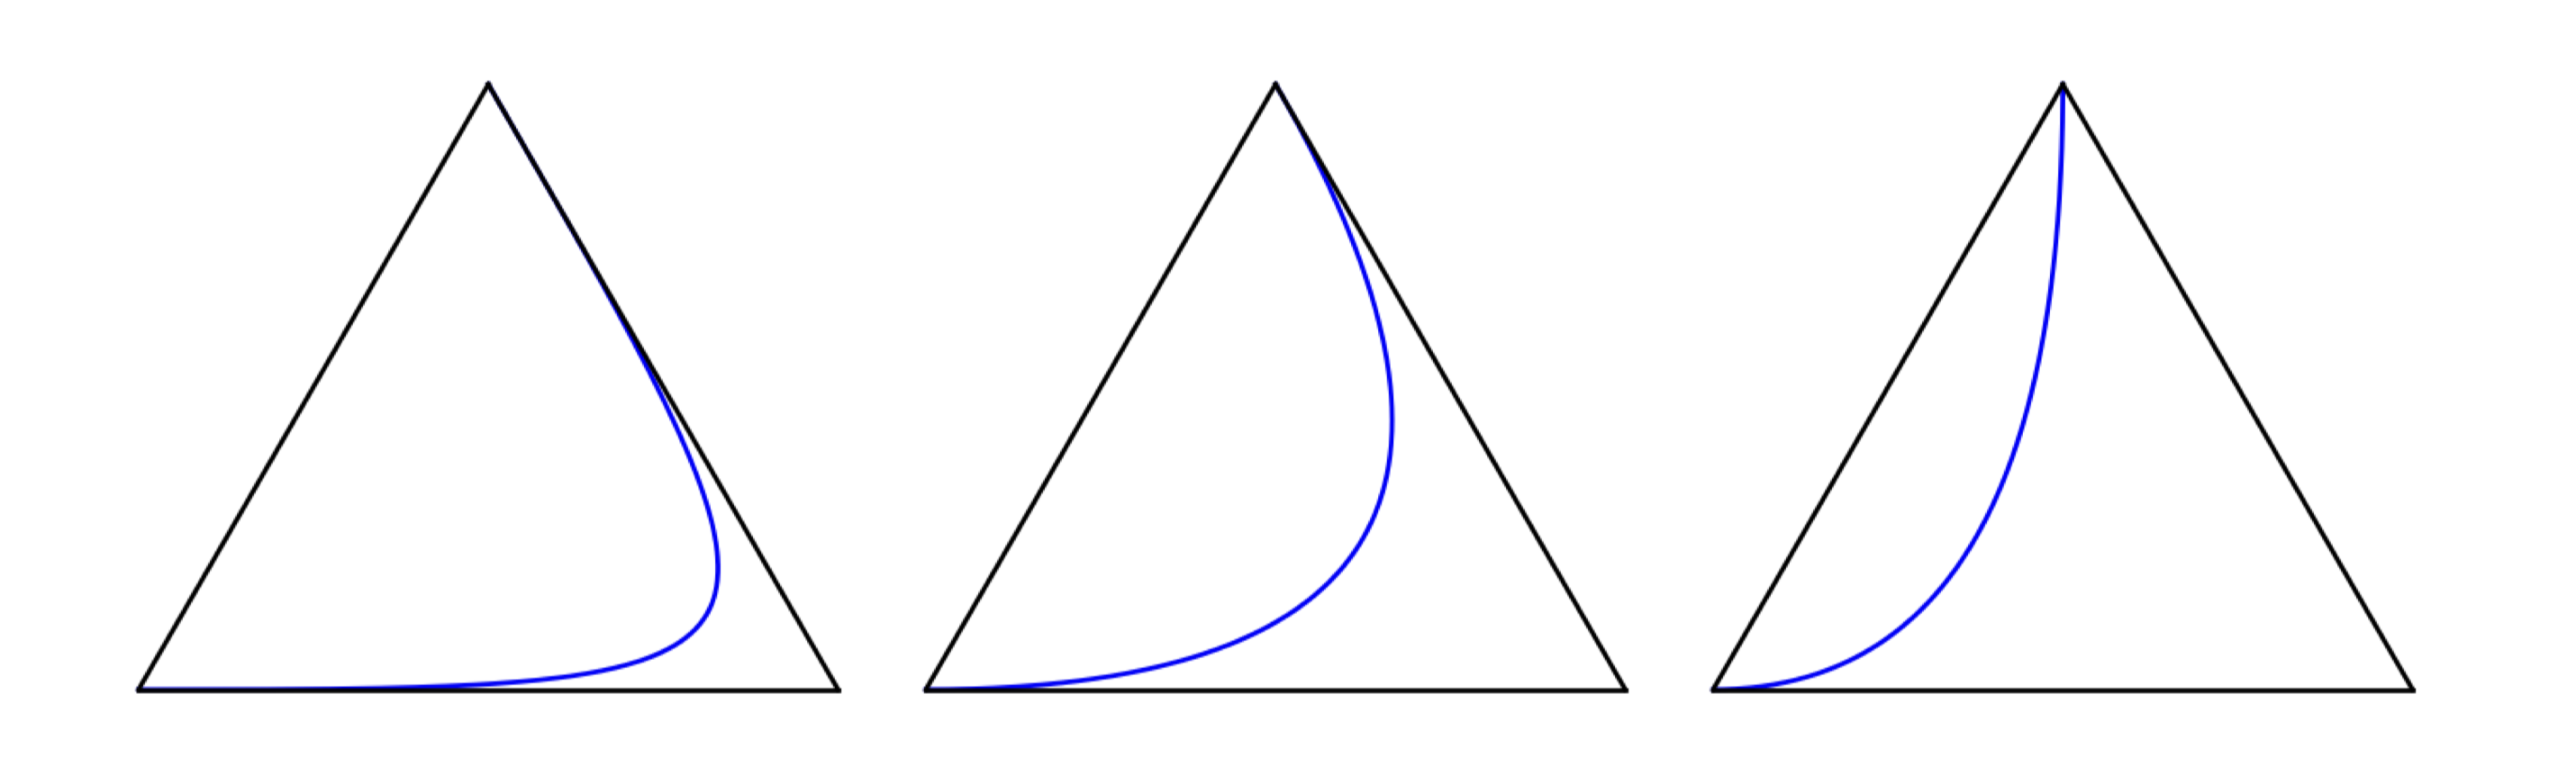
\includegraphics[width=0.8\textwidth]{assets/fundamental-models-delta-2.png}
    \caption{From left to right the illustration depicts the models parametrized \( ((1-\theta)^3, 3\theta(1-\theta), \theta^3) \), \( ((1-\theta)^2, 2\theta(1-\theta), \theta^2) \), \( (1-\theta, \theta(1-\theta), \theta^2) \), and \( ((1-\theta)^2, \theta, \theta(1-\theta)) \). The illustration is taken from \cite{bik2022classifying}.}
\end{figure}

We just computed all fundamental models of degree three or less in \( \Delta_2 \). We will see shortly that these are all models in the probability simplex \( \Delta_2 \). Of course, \( \Delta_2 \) contains non-reduced models, too. These are models that come from linear embeddings \( \Psi_{\lambda,k} \) and \( \Psi_{\lambda,k,h} \), see Proposition \ref{prop:linear-embedding-1} and Proposition \ref{prop:linear-embedding-2}. There are infinitely many of them, and for \( \lambda = \frac{1}{3} \) we obtain the models \( \theta \mapsto (\frac{2}{3}\theta, \frac{1}{3}, \frac{2}{3}(1 - \theta)) \) and \( \theta \mapsto (1-\theta, \frac{1}{3}\theta, \frac{2}{3}\theta) \).

\begin{figure}[H]
    \centering
    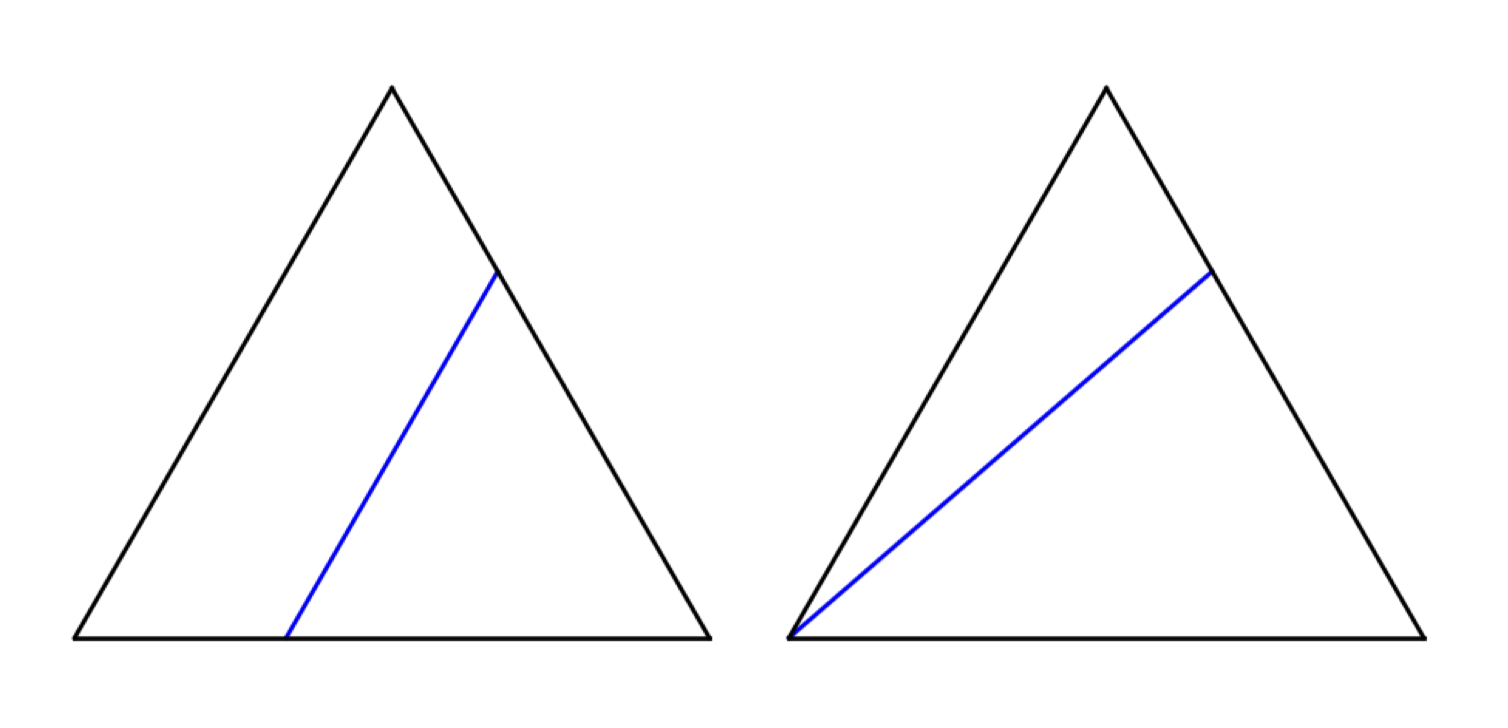
\includegraphics[width=0.66\textwidth]{assets/non-red-models-delta-2.png}
    \caption{This illustration depicts two non-reduced models in \( \Delta_2 \) for \( \lambda = \frac{1}{3} \). They are parametrized by \( \theta \mapsto (\frac{2}{3}\theta, \frac{1}{3}, \frac{2}{3}(1 - \theta)) \) and \( \theta \mapsto (1-\theta, \frac{1}{3}\theta, \frac{2}{3}\theta) \). All other non-reduced models can be obtained by varying \( \lambda \). The illustration is taken from \cite{bik2022classifying}.} 
\end{figure}
\end{example}

Let us summarize the results of this section. It is the first part of our classification theorem.

\begin{theorem}\label{thm:classification-jekns}
    Every one-dimensional discrete statistical model with rational MLE in \( \Delta_n \) is the image of a reduced model in \( \Delta_m \) under a linear embedding \( \Delta_m \to \Delta_n \) for some \( m \leq n \).

    Moreover, every reduced model \( \mathcal{M} \subset \Delta \) can be written as a composite of finitely many fundamental models
    \begin{align*}
        \mathcal{M} = \mathcal{M}_1 *_{\mu_1} ( \dots *_{\mu_{m-2}}( \mathcal{M}_{m-1} *_{\mu_{m-1}} \mathcal{M}_m) )
    \end{align*}
    for some \( m < n \) and \( \mu_1, \dots, \mu_m \in (0,1) \).
\end{theorem}

\begin{proof}
    See Proposition \ref{prop:composition-fundamental}, Proposition \ref{prop:linear-embedding-1}, and Proposition \ref{prop:linear-embedding-2}.
\end{proof}

\section{On the Finiteness of Fundamental Models}

We have established the first part of our classification theorem, namely that fundamental models are building blocks for all models. The second part is showing that there are only finitely many fundamental models in \( \Delta_n \) given \( n \in \mathbb{N} \). Artuhr Bik and Orlando Marigliano proved that there are only finitely many fundamental models in \( \Delta_n \) for \( n \leq 4 \) \cite{bik2022classifying}. We will later make significant progress towards proving the case \( n = 5 \). For \( n \geq 6 \) no attempt has been made yet to the best of our knowledge.

Arthur Bik and Orlando Marigliano first proved the following proposition.

\begin{theorem}\label{thm:degree-fundamental-models}
    Let \( \mathcal{M} \) be a one dimensional discrete statistical model with rational MLE in \( \Delta_n \). For \(n \leq 4 \) we have \( \mathrm{deg}(\mathcal{M}) \leq 2n - 1\).
\end{theorem}

Given Theorem \ref{thm:degree-fundamental-models} it is easy to show the second part of our classification.

\begin{theorem}\label{thm:finiteness-fundamental-models}
    There are only finitely many fundamental models in \( \Delta_n \) for all \( n \leq 4 \).
\end{theorem}

\begin{proof}
    By Theorem \ref{thm:degree-fundamental-models} we know that the degree of a fundamental model is at most \( 2n - 1 \). Since the number of supports of a fundamental model of degree \( 2n - 1 \) is finite, there are only finitely many fundamental models in \( \Delta_n \) for all \( n \leq 4 \).
\end{proof}

We will now spend the rest of this thesis on proving Theorem \ref{thm:degree-fundamental-models}. The idea is to use the building blocks of fundamental models that we have established so far. Namely, it suffices to show the theorem for fundamental models.

\begin{theorem}\label{thm:degree-fundamental-models-reduced}
    Let \(N \in \mathbb{N} \). If for all $n \leq N$ and for all fundamental models \( \mathcal{M} \in \Delta_n\) the upper bound \( \mathrm{deg}(\mathcal{M}) \leq 2n - 1\)  holds, then the upper bound also holds for all statistical models in \( \Delta_{n'} \) for all \( n' \leq N \).    
\end{theorem}

\begin{proof}
    Let $N \in \mathbb{N}$ and $n \leq N$.
    Assume there is some non-fundamental model $\mathcal{M}'$ in $\Delta_n$ of degree greater than $2n - 1$. By Corollary \ref{cor:fundamental-models-ksmlkdf} there exists a fundamental model $\mathcal{M}$ in $\Delta_m$ for some $m < n$ of degree greater than $2m - 1$. This contradicts the assumption that the degree of fundamental models is at most $2n' - 1$ for all $n' \leq N$.
\end{proof}

Counting all \emph{fundamental} models in $\Delta_n$ for $n \leq 4$ is our guiding objective. As a first step, we introduce a combinatorial game that aids in counting fundamental models. We know that every reduced model can be represented by the sequence of triples $(w_k, i_k, j_k)^{n}_{k=0}$, where $w_k \in \mathbb{R}_{>0}$ and $i_k, j_k \in \mathbb{Z}_{\geq 0}$. The model can be visualized in a directed graph with vertices in $\mathbb{Z}^2$, where we can place values $w_k$ on vertices $(i_k, j_k)$. Each vertex $(i,j)$ is connected by directed edges to $(i+1, j)$ and $(i, j+1)$. 

\begin{figure}\label{fig:binom-discrete-model-visual}
    \centering
    % https://tikzcd.yichuanshen.de/#N4Igdg9gJgpgziAXAbVABwnAlgFyxMJZABgBoBmAXVJADcBDAGwFcYkQA6EAX1PU1z5CKMgCZqdJq3Zde-bHgJEAjBQkMWbRJx58QGBUKJll6qVpDLd8wUpSrxNDdO2jr+gYuHJRap+fYrOQ9DO2RVU39NGXcDW29fSMlo7Vk9OK8iX0dklx1gjKMUcj9cizSbTOLSHOdy2M8i5BKkupiCxrCS4jMU-PTOhNIeqLyKkPiVYd6xhtDvMhGy9okYKABzeCJQADMAJwgAWyQyEBwIJGVg-aOTmnOkUWuD48RfM4vEAFZn27f7z4AFl+r1UHyQwL0N1BAKQ5BBcNhiGUPyhL0uXyRykhu3RiAAbFicSBoRCkfiEQSkQB2SnYrHwtF-akMyks8HIq5M0ElDnKJ7cy5gh7IgW4v6ApEADkpUpplMxHIAnArpbKscQ6acRcoueLXkqNZTeSKKZRuEA
    \begin{tikzcd}
        . \arrow[r]           & . \arrow[r]           & . \arrow[r]           & .           \\
        1 \arrow[u] \arrow[r] & . \arrow[u] \arrow[r] & . \arrow[u] \arrow[r] & . \arrow[u] \\
        . \arrow[r] \arrow[u] & 2 \arrow[u] \arrow[r] & . \arrow[u] \arrow[r] & . \arrow[u] \\
        . \arrow[u] \arrow[r] & . \arrow[r] \arrow[u] & 1 \arrow[r] \arrow[u] & . \arrow[u]
    \end{tikzcd}
    \caption{The binomial model with two trials visualized in a directed graph with vertices in $\left\{0,1,2,3 \right\}^2$.}
\end{figure}


Surprisingly, we can derive a combinatorial game from this graph by defining a specific set of rules. This game, called the \emph{chipsplitting game}, will be rigorously introduced in the next chapter. After that, we will explore the game's properties and show how it can be used to count fundamental models in $\Delta_n$ for $n \leq 4$.